\section{Seguimiento longitudinal}

\subsection{Resumen de entradas y salidas del SPS}

\begin{table}[!htbp]
\centering
\begin{minipage}{0.5\textwidth}
  \centering
  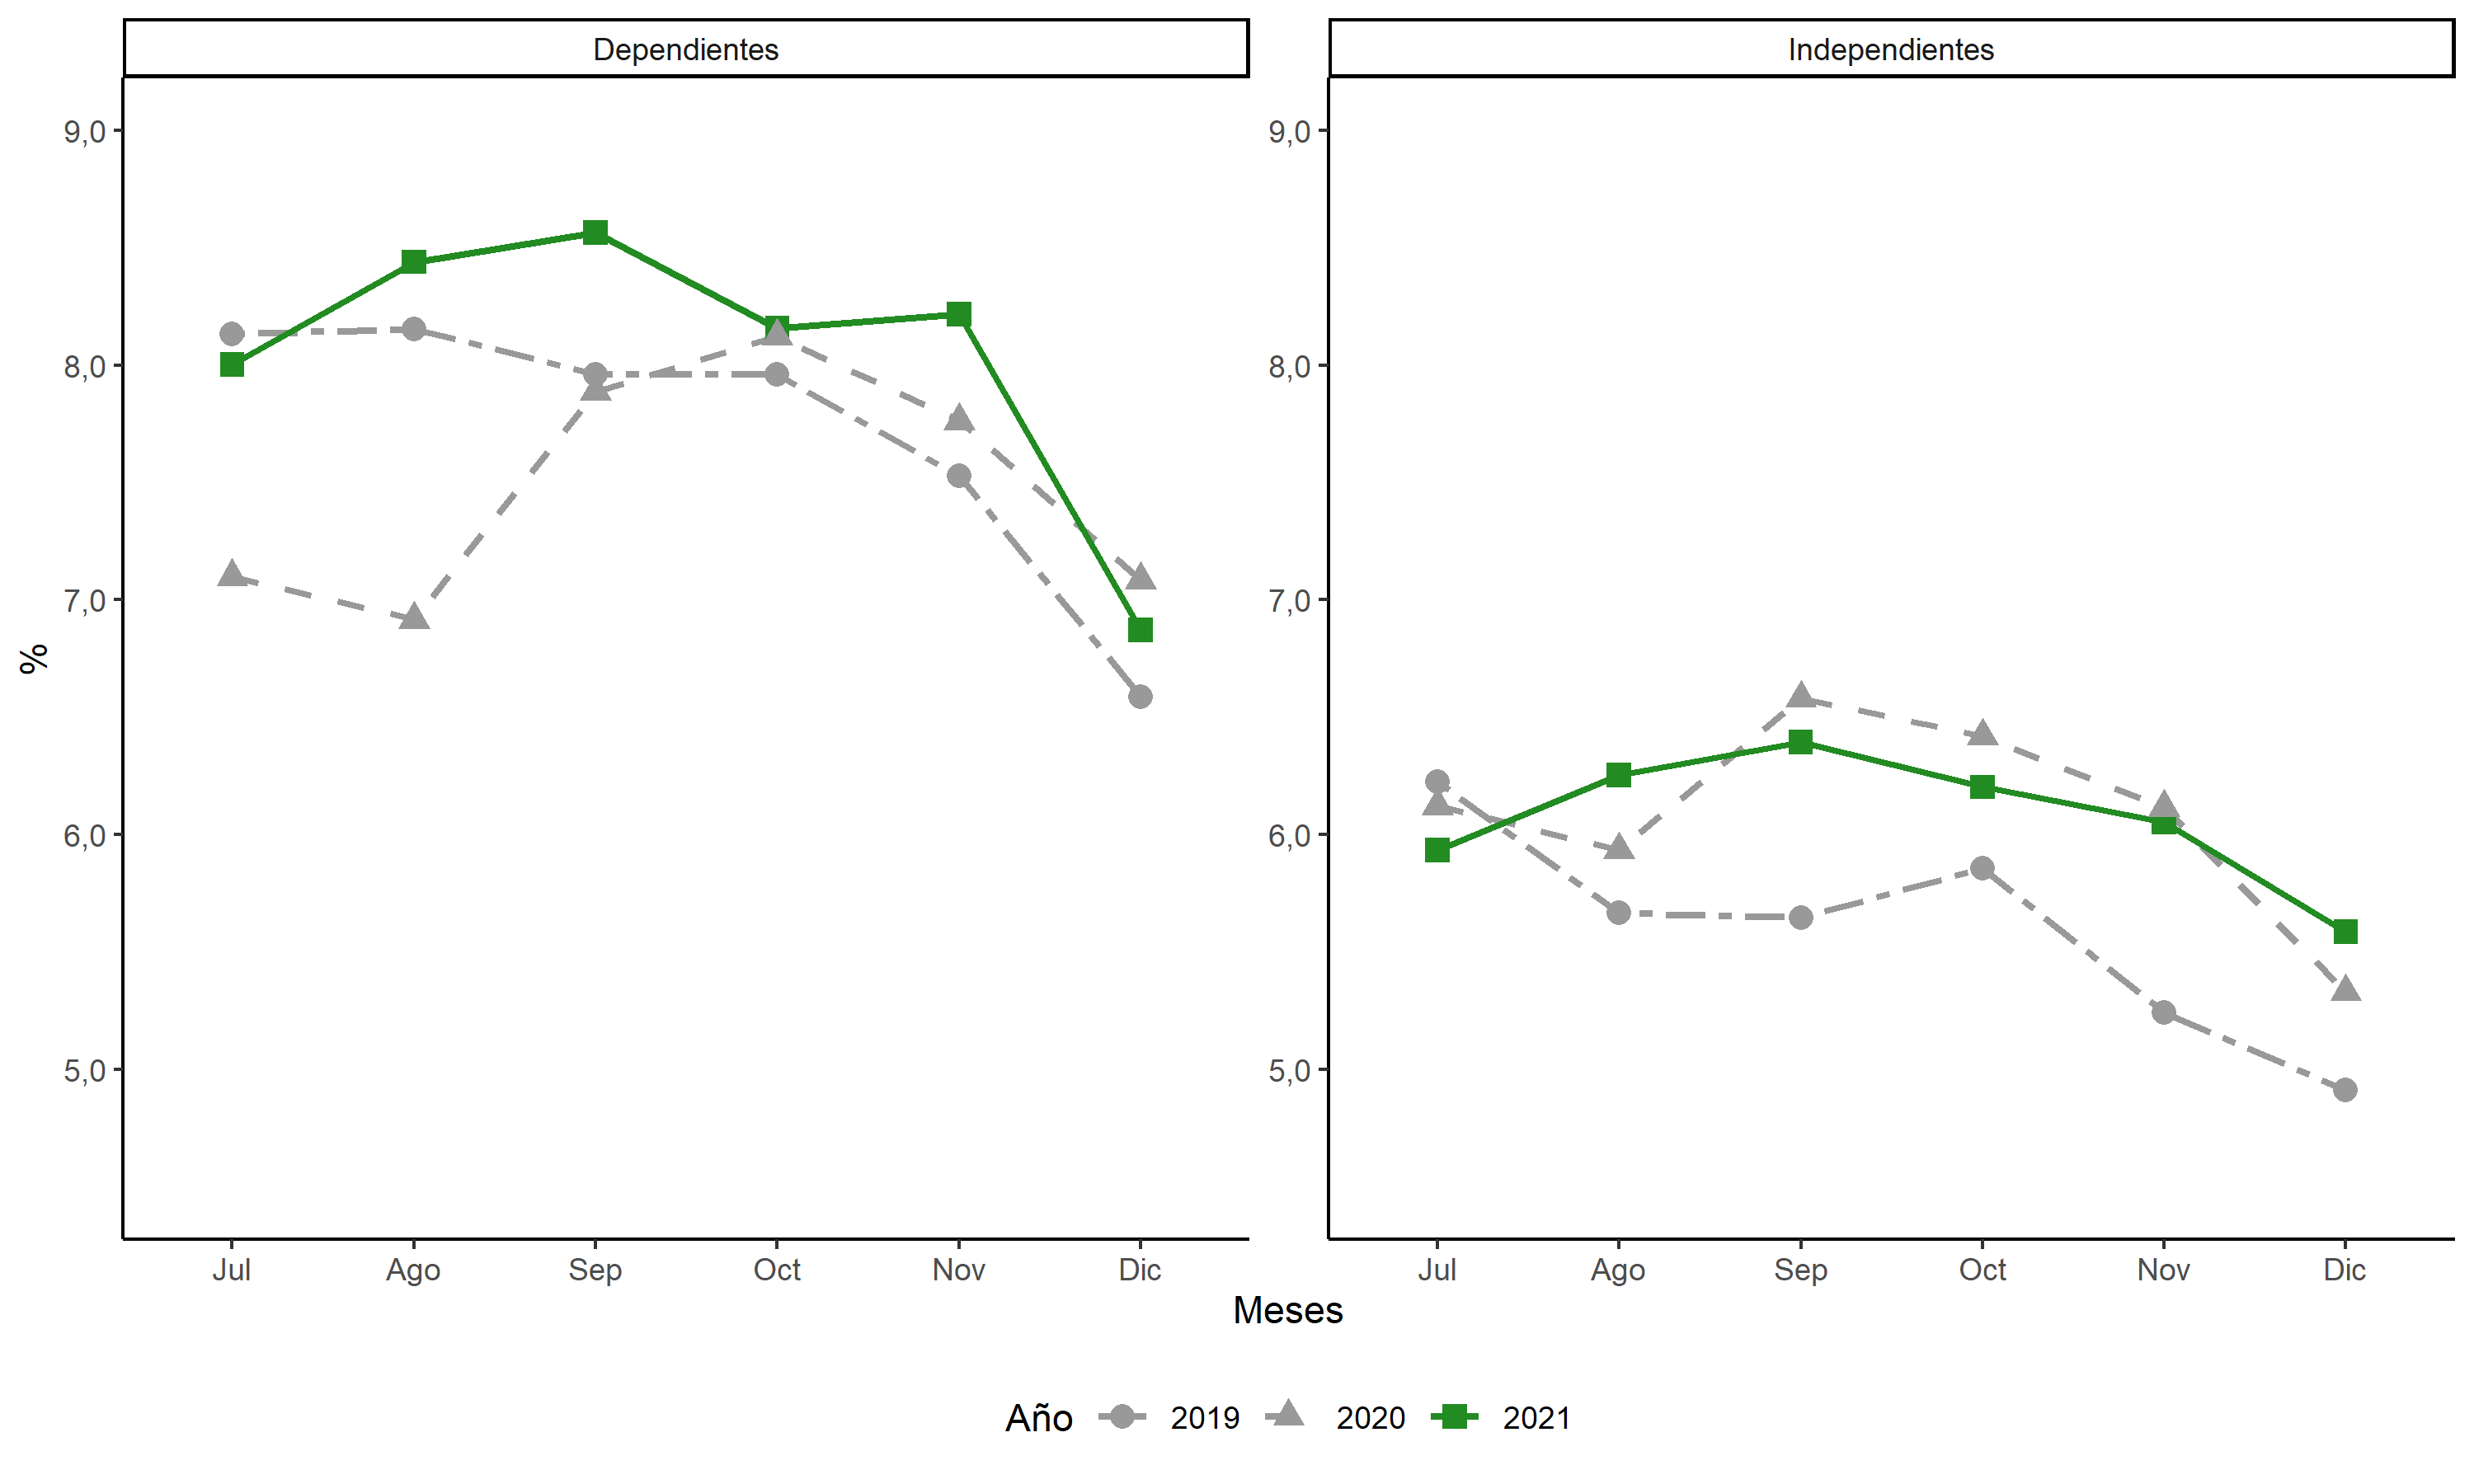
\includegraphics[width=\linewidth]{figures/02_longitudinal/entradas_anual_dependiente_independiente.png}
\end{minipage}%
\begin{minipage}{0.5\textwidth}
  \centering
  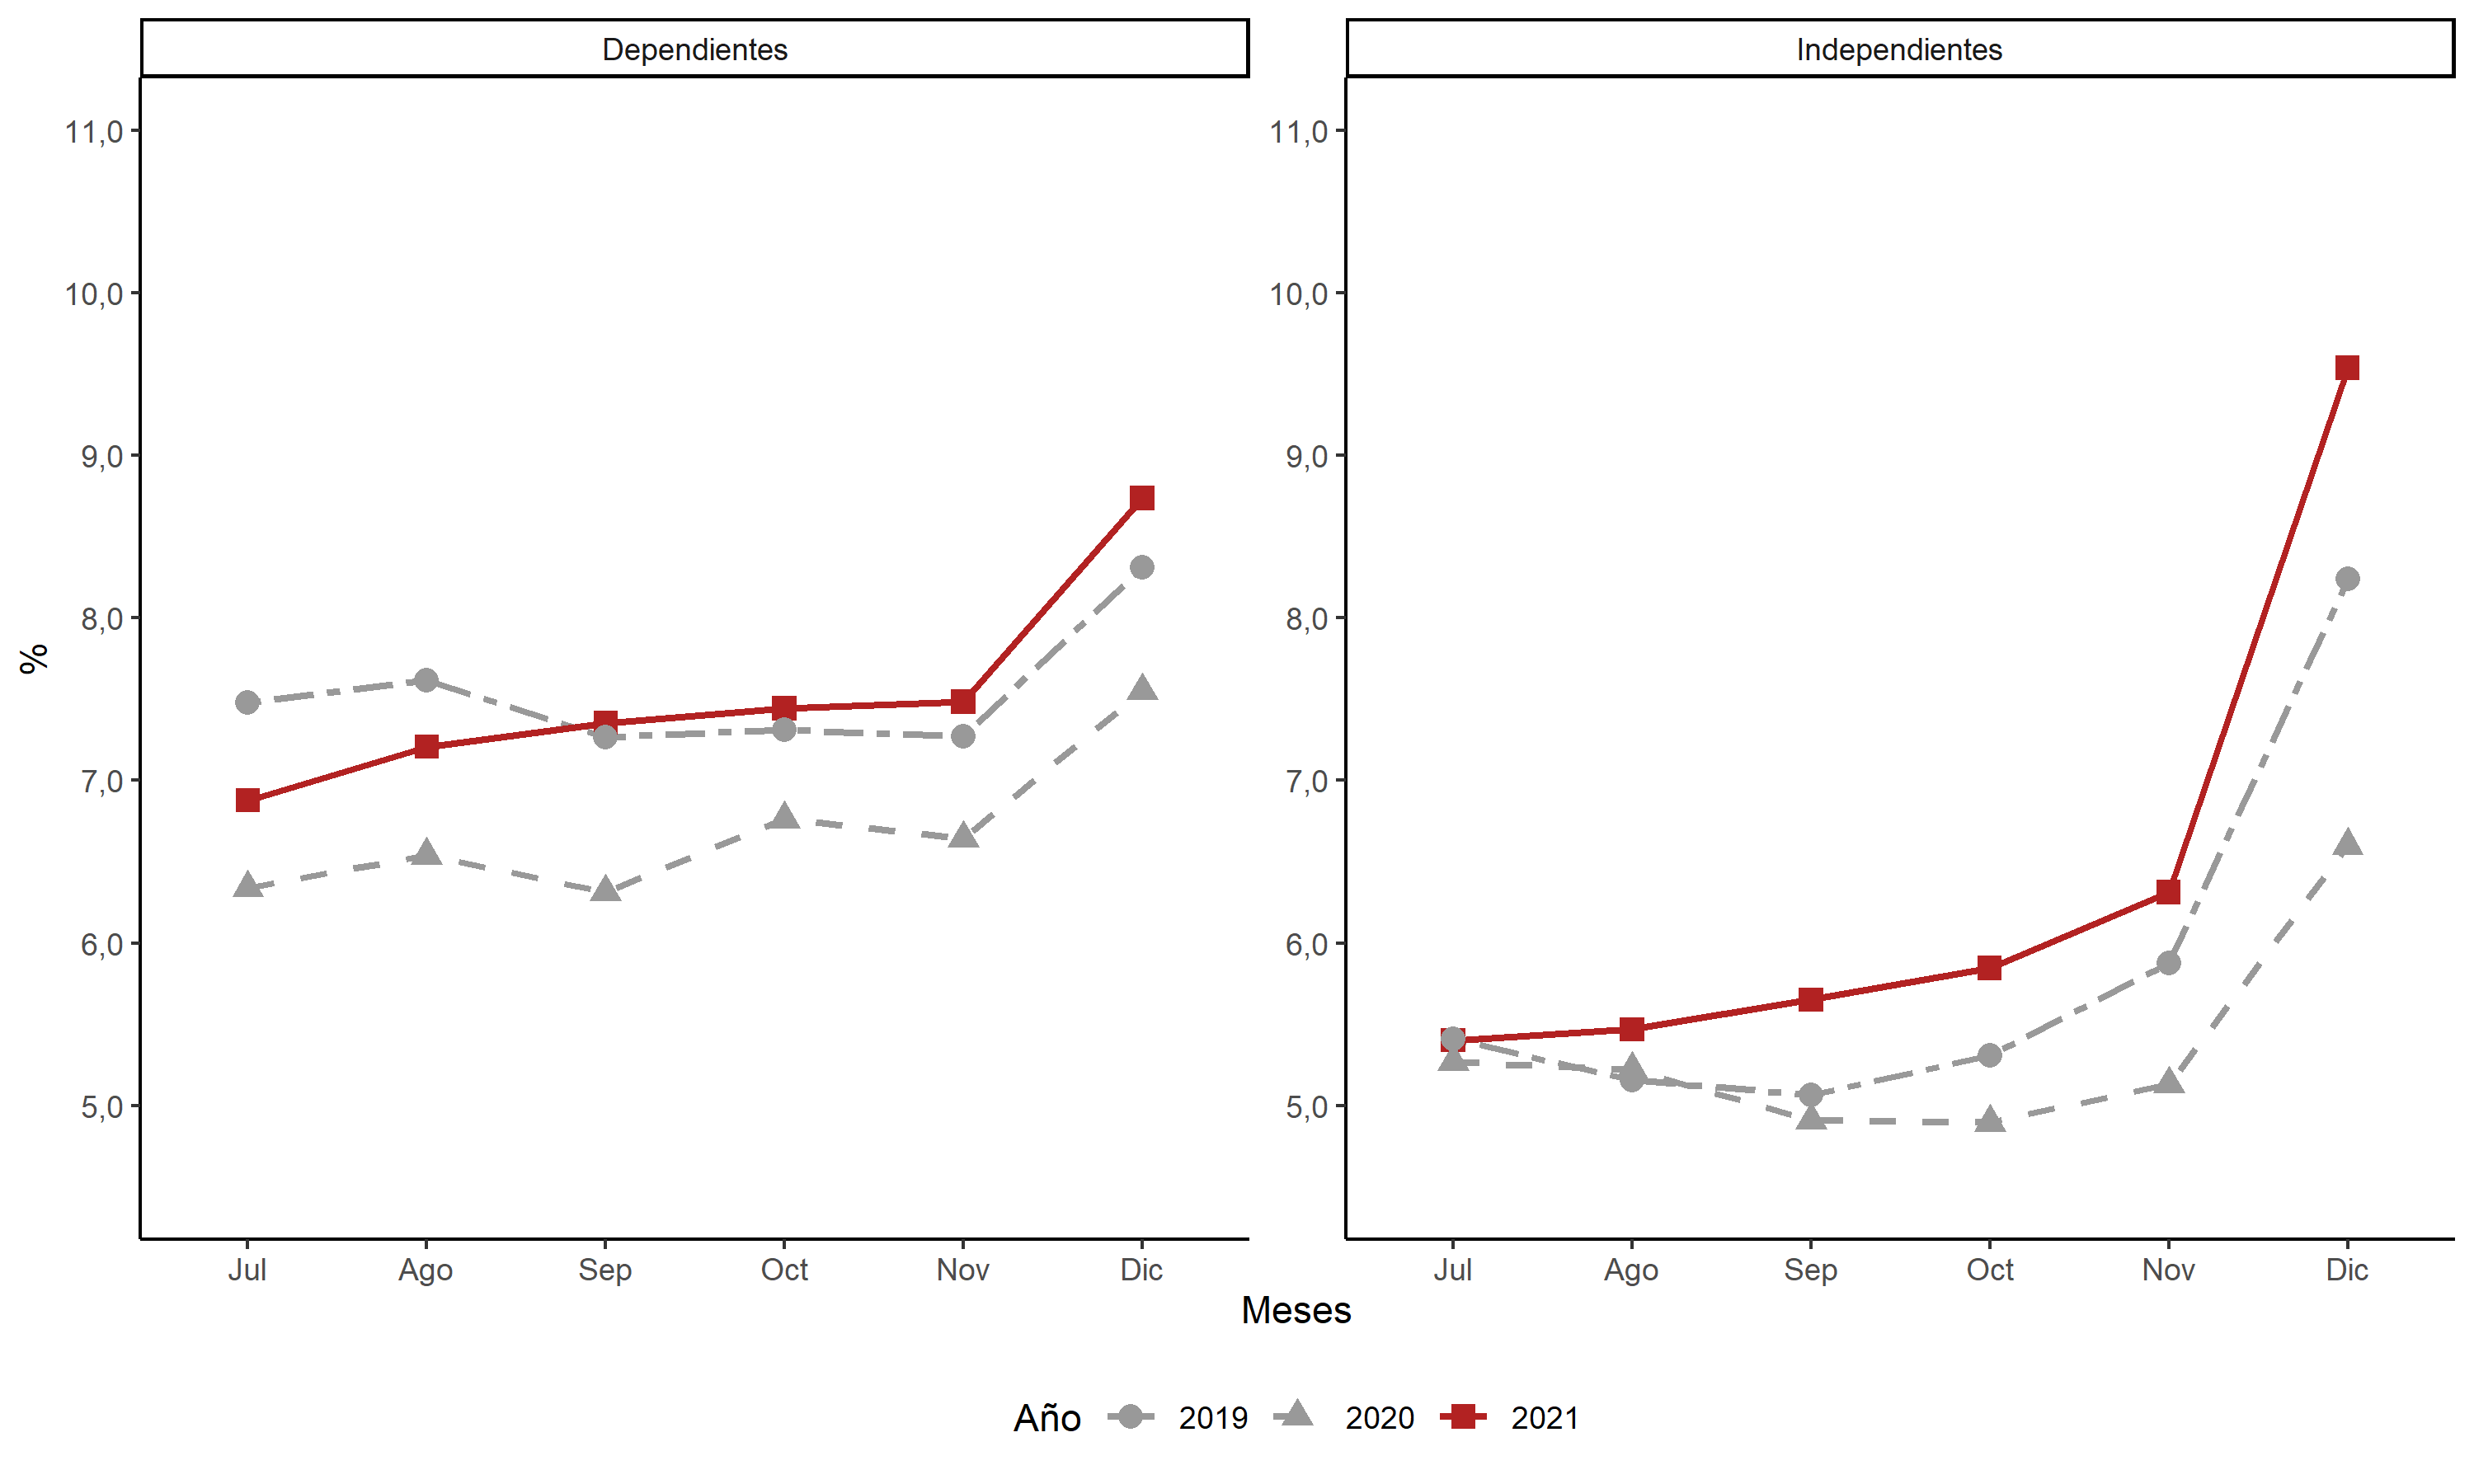
\includegraphics[width=\linewidth]{figures/02_longitudinal/salidas_anual_dependiente_independiente.png}
\end{minipage}
\caption{Porcentaje de entradas (izq.) y salidas (der.) por año)}
\label{tabla:dependientes:entradas_salidas}
\end{table}

\FloatBarrier
\subsection{Cotizantes dependientes del Sector privado}
\subsubsection{Dinámica de entradas y salidas del SPS}
En diciembre 2021 entraron\footnote{los \textbf{ingresos} corresponden a las relaciones laborales que no se encuentran en el periodo previo pero ahora si las vemos}, permanecieron\footnote{las \textbf{permanencias} corresponden a las relaciones laborales que se encuentran en el periodo de análisis y el periodo previo} y salieron\footnote{las \textbf{salidas} corresponden a las relaciones laborales que no se encuentran en el periodo de análisis y si en el periodo previo} 598.204, 8.106.864 y 776.052 relaciones laborales dependientes del sector privado. Las entradas superan en 22.940 y 46.784 las entradas en 2020 y 2019, las salidas en este periodo también supera a las de 2020 y 2019 en 159.722 y 67.120 relaciones laborales. 


Las entradas en diciembre 2021 corresponden al 6.8\% de las relaciones laborales en este periodo siendo inferior al observado en 2020 y superior al obtenido en 2019 que fueron del 7.08\% y 6.5\%. Las dinámicas en rangos inferiores a los 2 Salarios Mensuales Mínimos Legales Vigentes (SMMLV) o menos son mas altos como se muestra en la tabla , las entradas de 1 SMMLV o menos son inferiores a los observados en 2020 y superiores a las observadas en 2019, que fueron del 16.3\% y 15.3\%, probablemente sea por el aumento de permanencias que aumentaron en 561.969 y en 288.017 con relación a relaciones laborales de 1 o menos SMMLV en 2020 y 2019 respectivamente. Por otro lado, las salidas son el 8.7\% de relaciones laborales en noviembre 2021, superando al porcentaje de salidas en 2020 y 2019 que fueron de 7.55\% y 8.31\% respectivamente. 

\begin{table}[!htbp]
\label{tabla:sector_privado:matriz_dinamica_mes_12_2021}
\centering
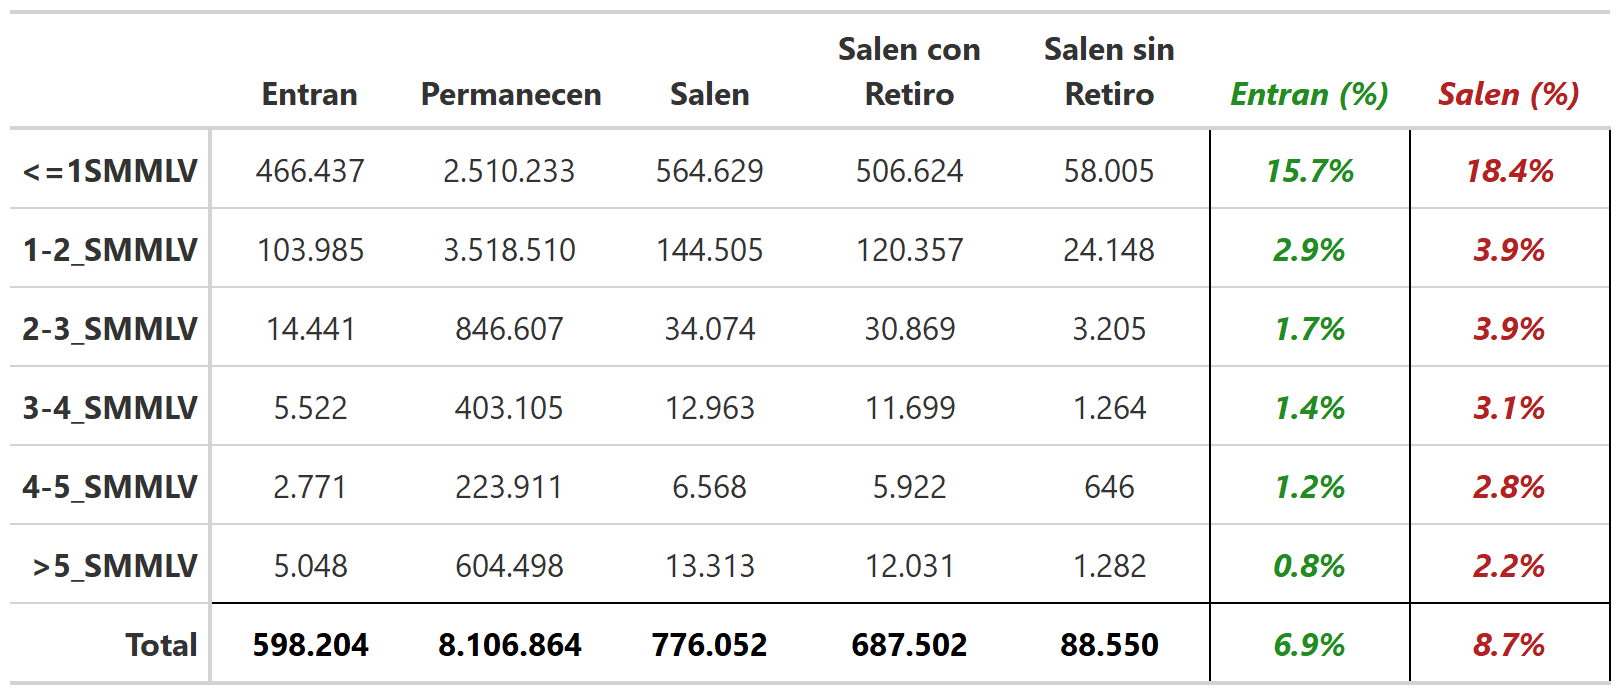
\includegraphics[width = 15cm]{results/02_longitudinal/salida_resumen_dependientes_interes_21.png}
\caption{Matriz dinámica pareada dependientes sector privado Noviembre - Diciembre 2021}%
\end{table}

\begin{table}[!htbp]
\label{tabla:sector_privado:matriz_dinamica_mes_11_2021}
\centering
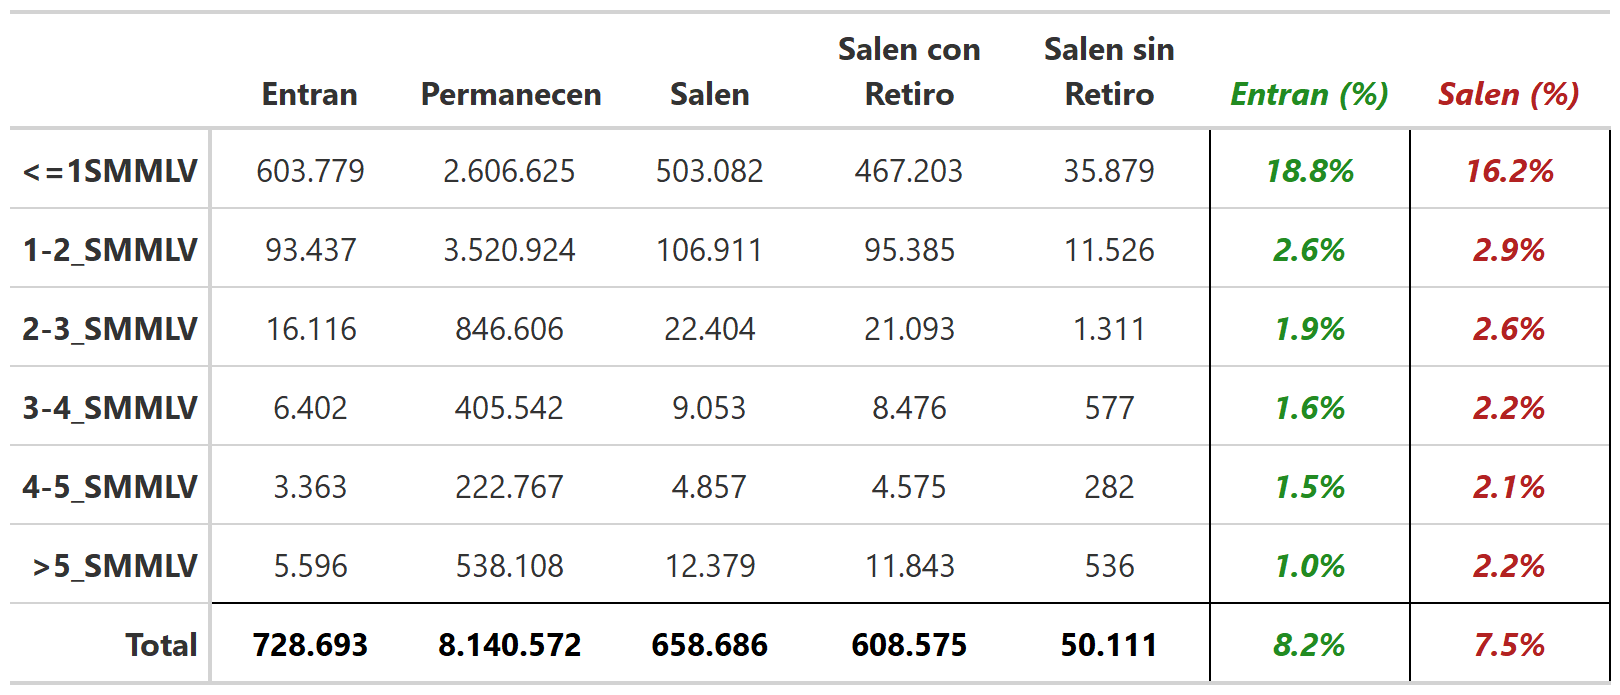
\includegraphics[width = 15cm]{results/02_longitudinal/salida_resumen_dependientes_referencia_21.png}
\caption{Matriz dinámica pareada dependientes sector privado Octubre - Noviembre 2021}%
\end{table}

%%%%%
\FloatBarrier
\paragraph{Relaciones laborales que permanecieron}\mbox{}\\

\begin{table}[!htbp]
\label{tabla:sector_privado:matriz_transicion_mes_11_12_2021}
\centering
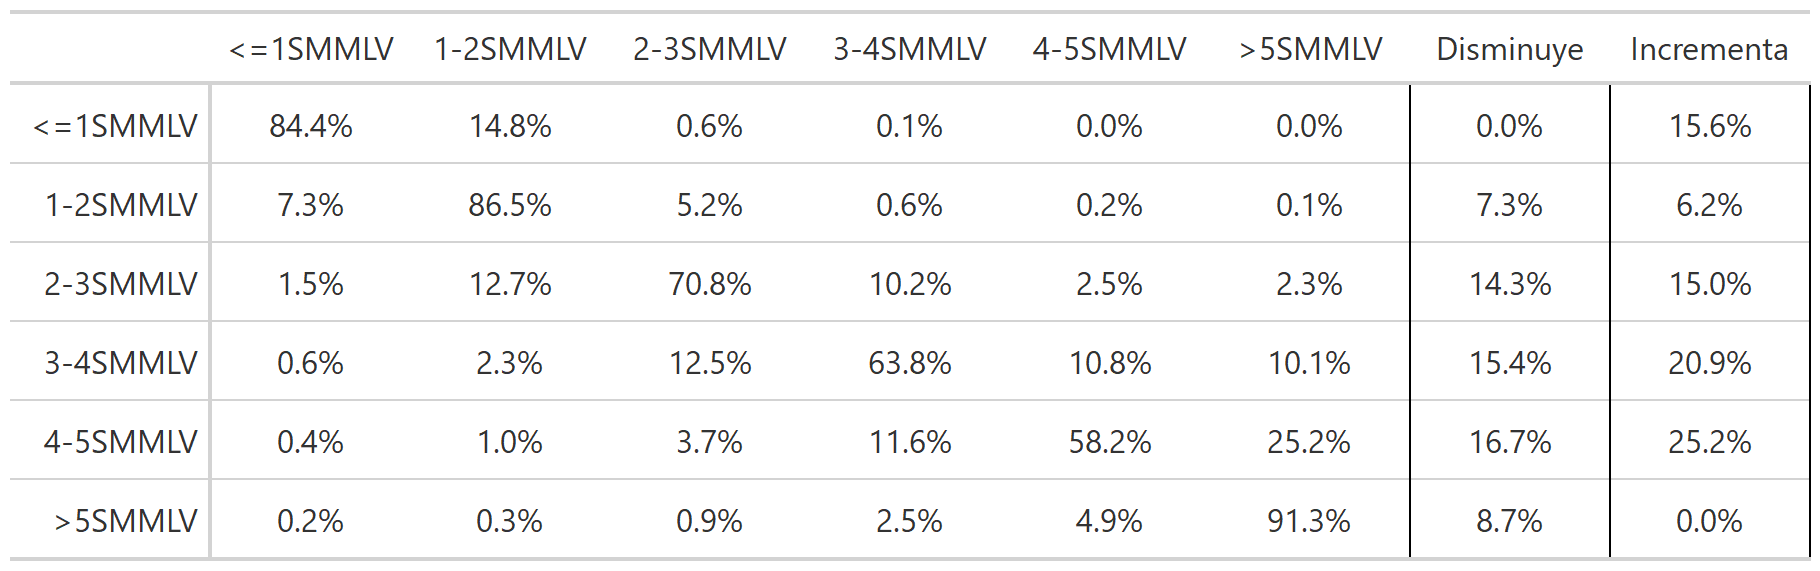
\includegraphics[width = 15cm]{results/02_longitudinal/salida_matriz_transicion_dependientes_21.png}
\caption{Matriz de transición sector privado Noviembre - Diciembre 2021}%
\end{table}

\FloatBarrier
\paragraph{Análisis por sección económica}\mbox{}\\

\begin{table}[!htbp]
\label{tabla:sector_privado:actividad_economica}
\centering
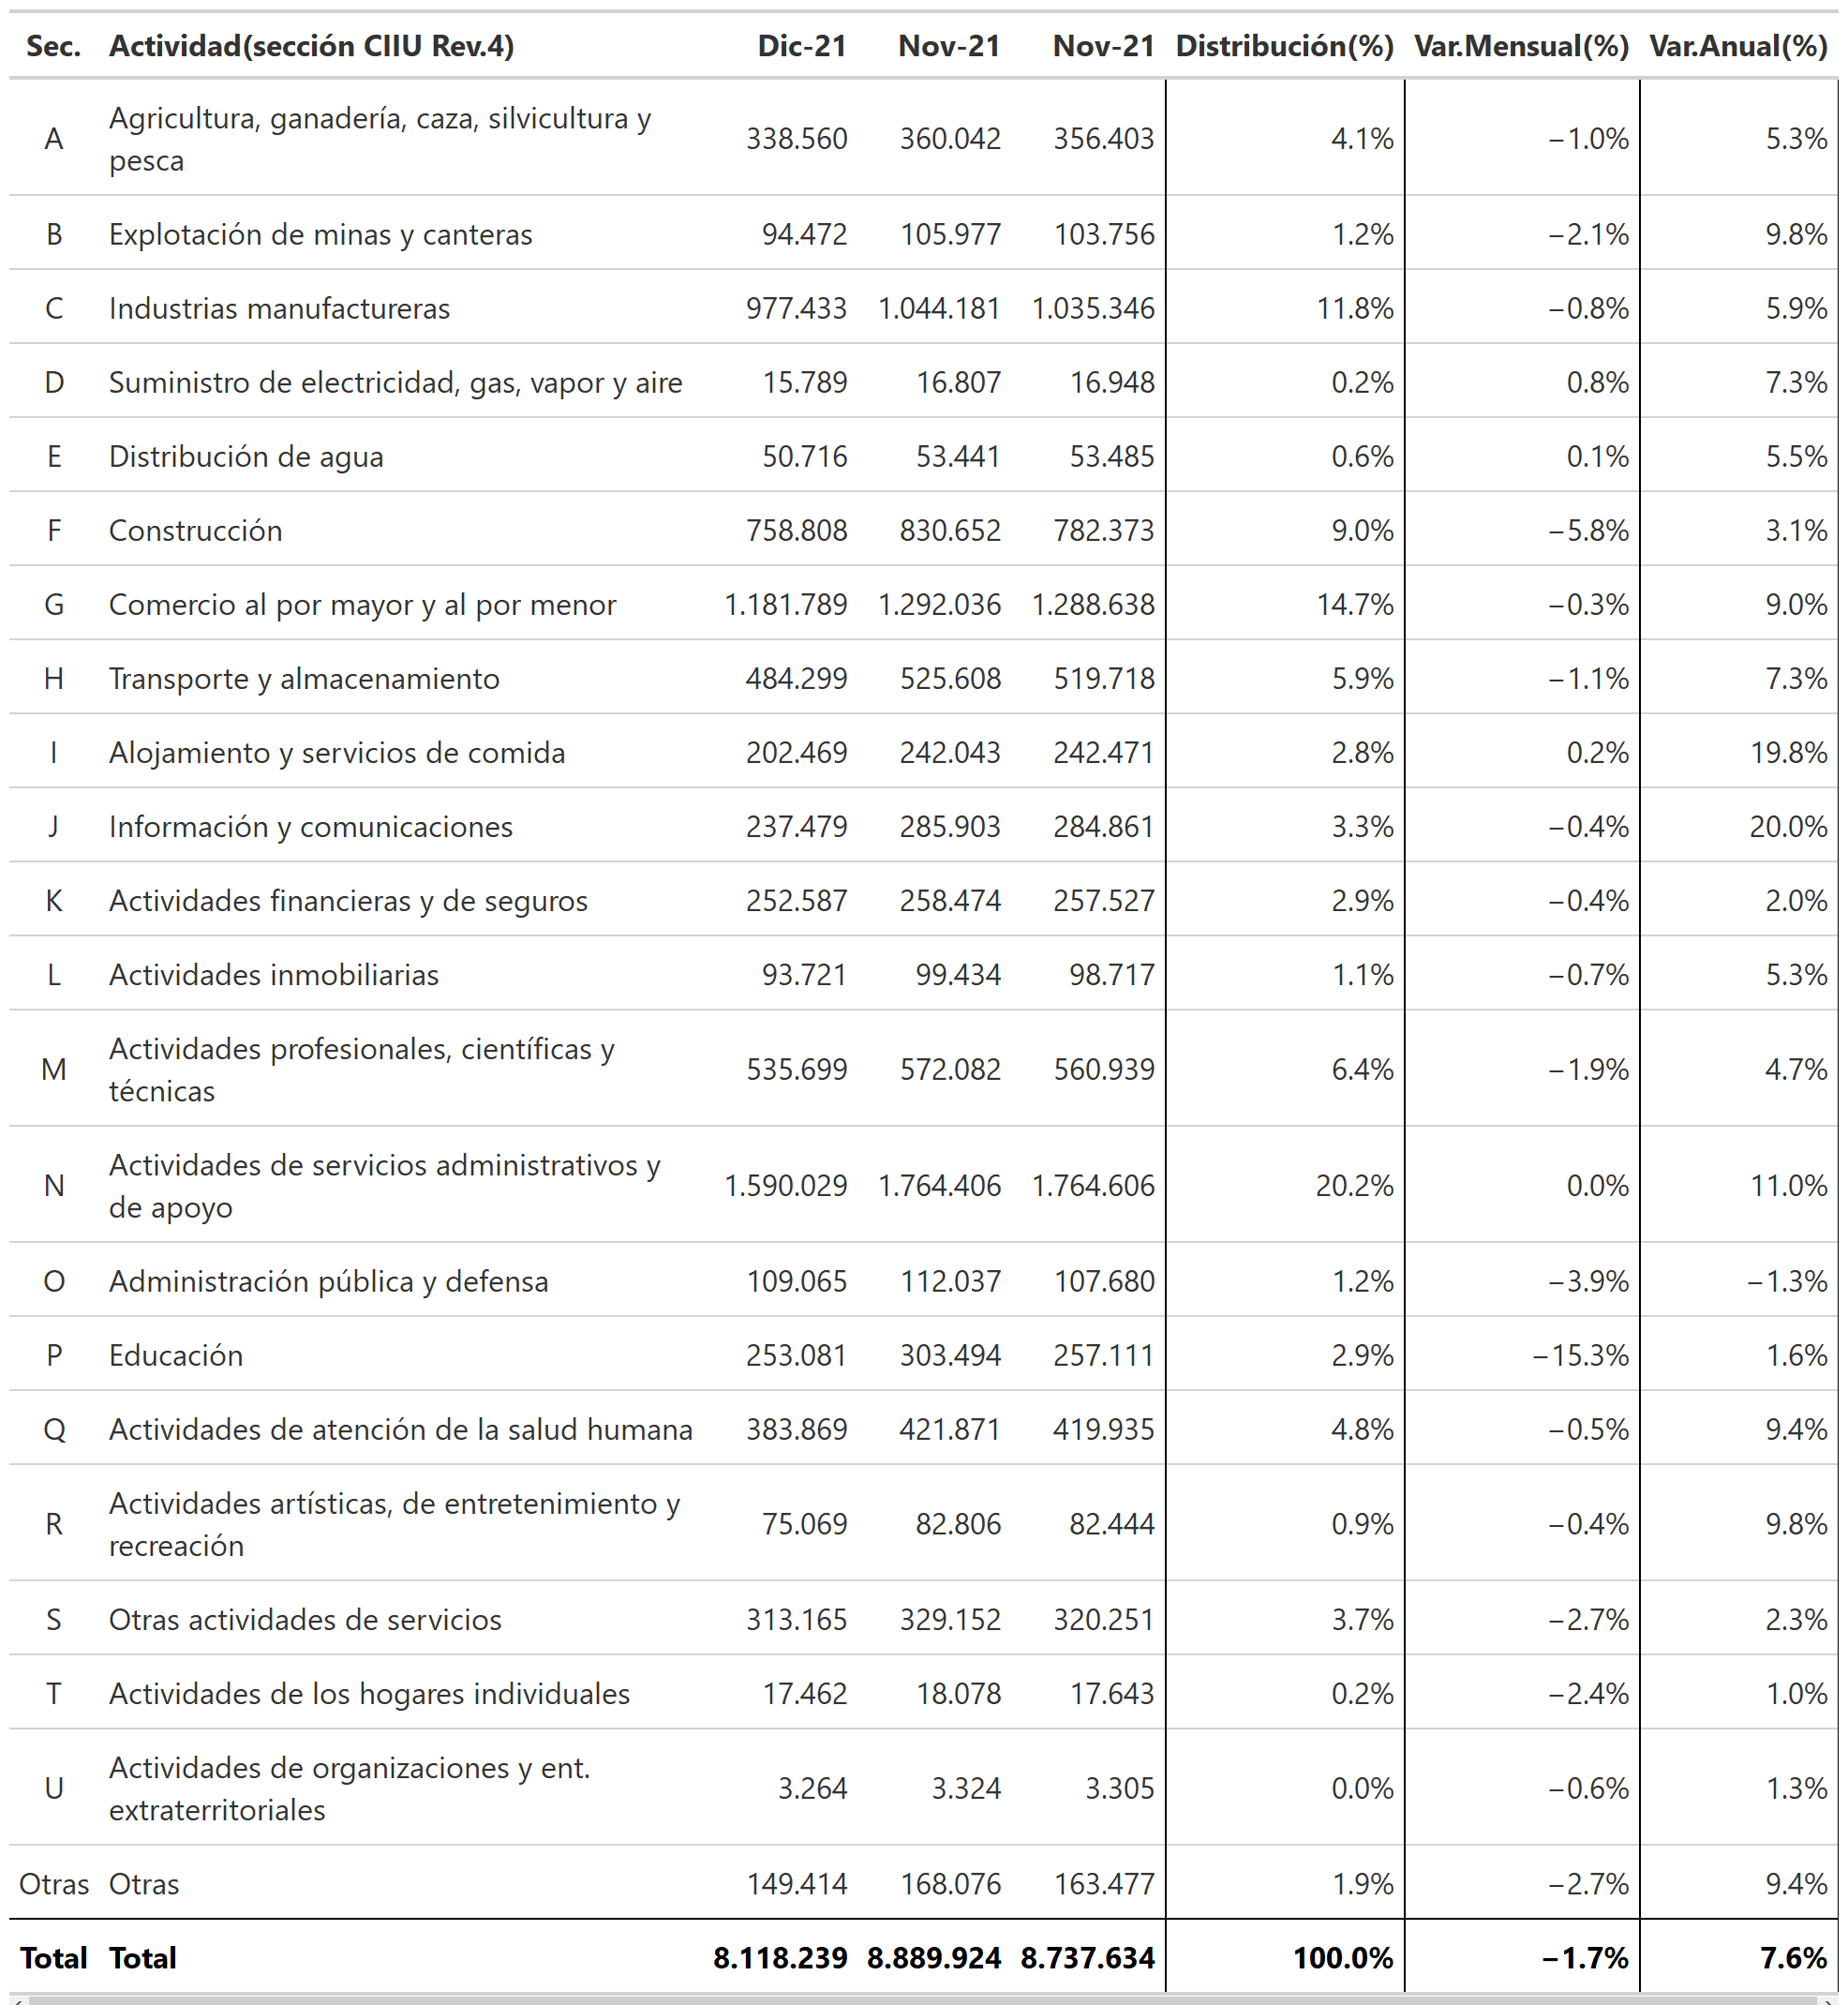
\includegraphics[width = 18cm]{results/02_longitudinal/salida_act_econ_dependientes_21.png}
\caption{Total cotizantes sector privado  por sección económica}%
\end{table}



%grfico 1 dinamicas del sector privado 
\FloatBarrier
\subsection{Independientes}

\subsubsection{Dinámica de entradas y salidas del SPS}
\begin{table}[!htbp]
\label{tabla:independientes:matriz_dinamica_mes_12_2021}
\centering
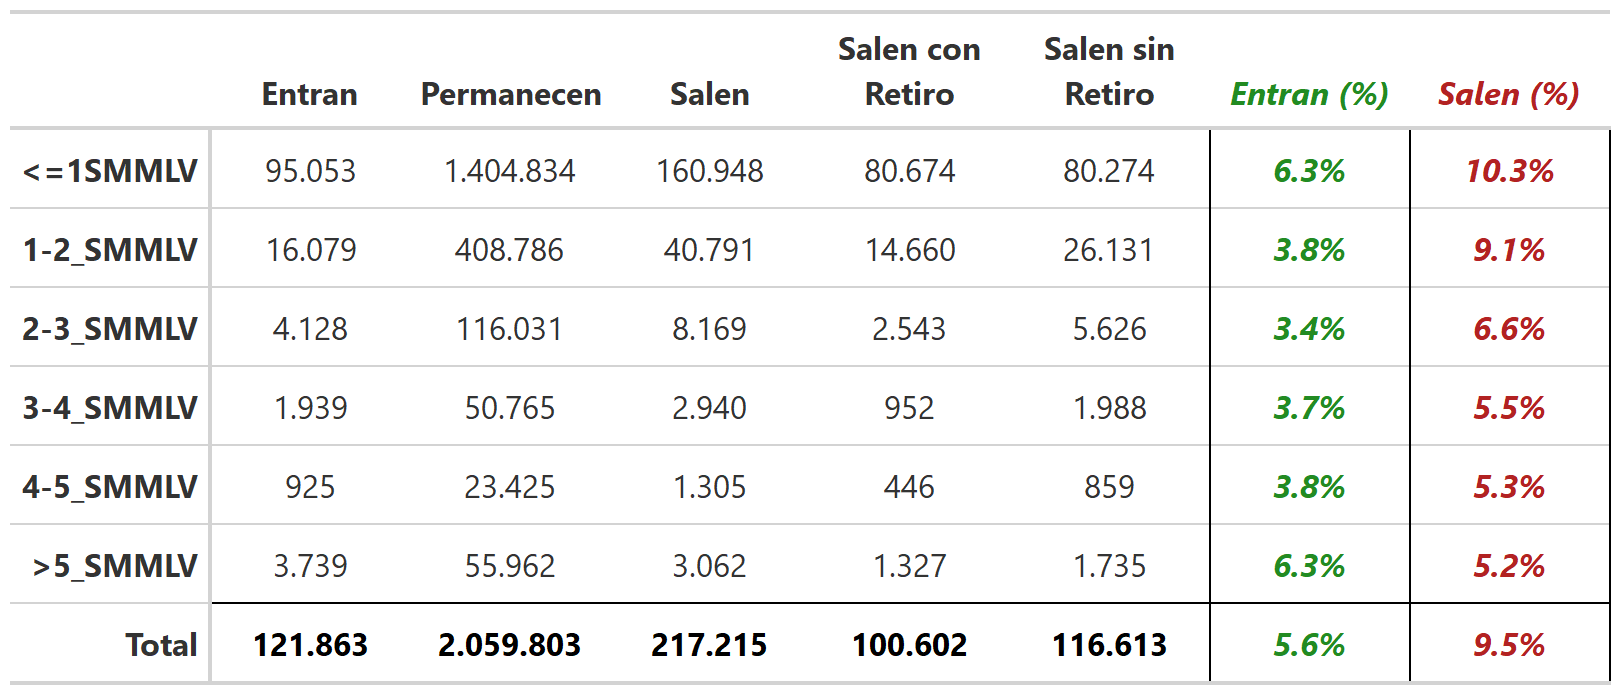
\includegraphics[width = 15cm]{results/02_longitudinal/salida_resumen_independientes_interes_21.png}
\caption{Matriz dinámica pareada independientes Noviembre - Diciembre 2021}%
\end{table}

\begin{table}[!htbp]
\label{tabla:independientes:matriz_dinamica_mes_11_2021}
\centering
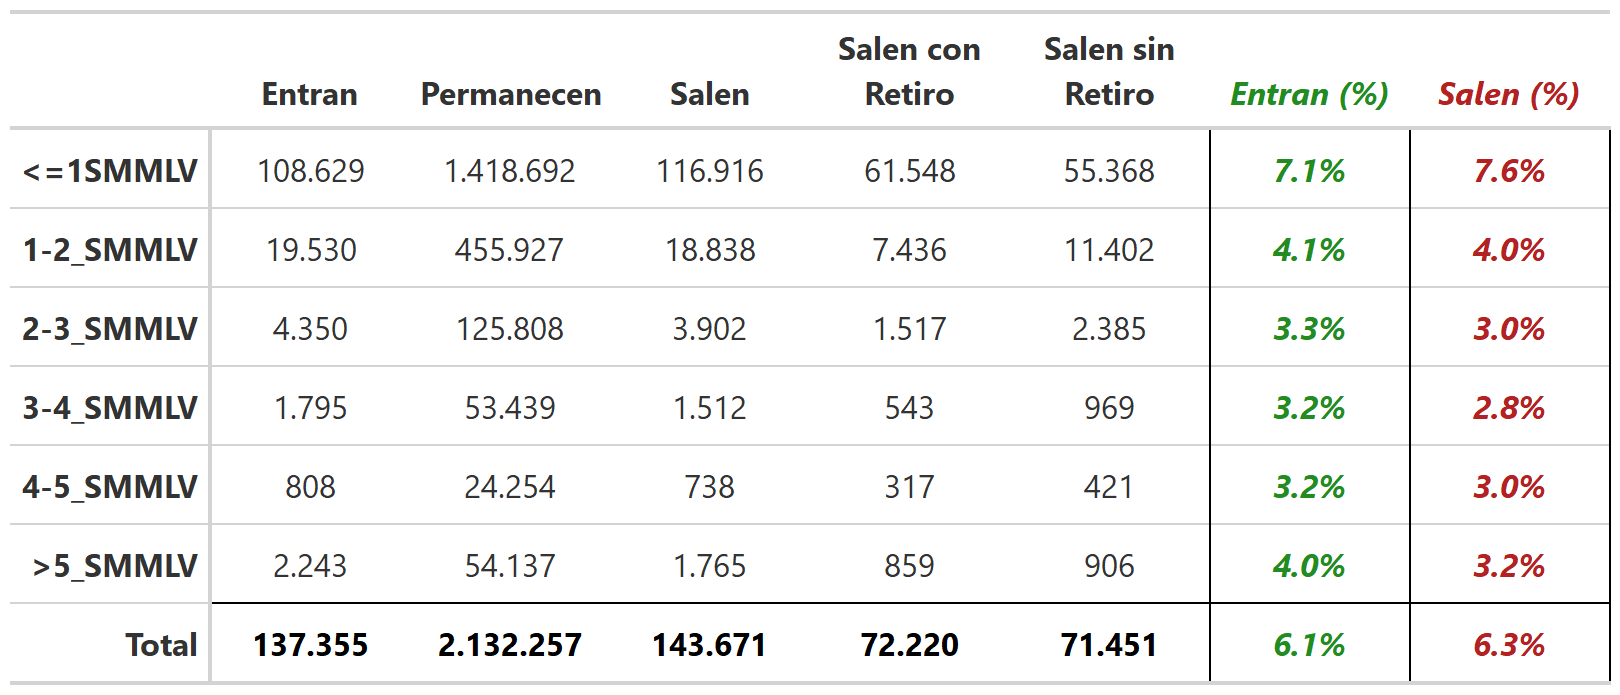
\includegraphics[width = 15cm]{results/02_longitudinal/salida_resumen_independientes_referencia_21.png}
\caption{Matriz dinámica pareada independientes Octubre - Noviembre 2021}%
\end{table}


\FloatBarrier
\paragraph{Relaciones laborales que permanecieron}\mbox{}\\


Las relaciones laborales que permanecieron 

\begin{table}[!htbp]
\centering
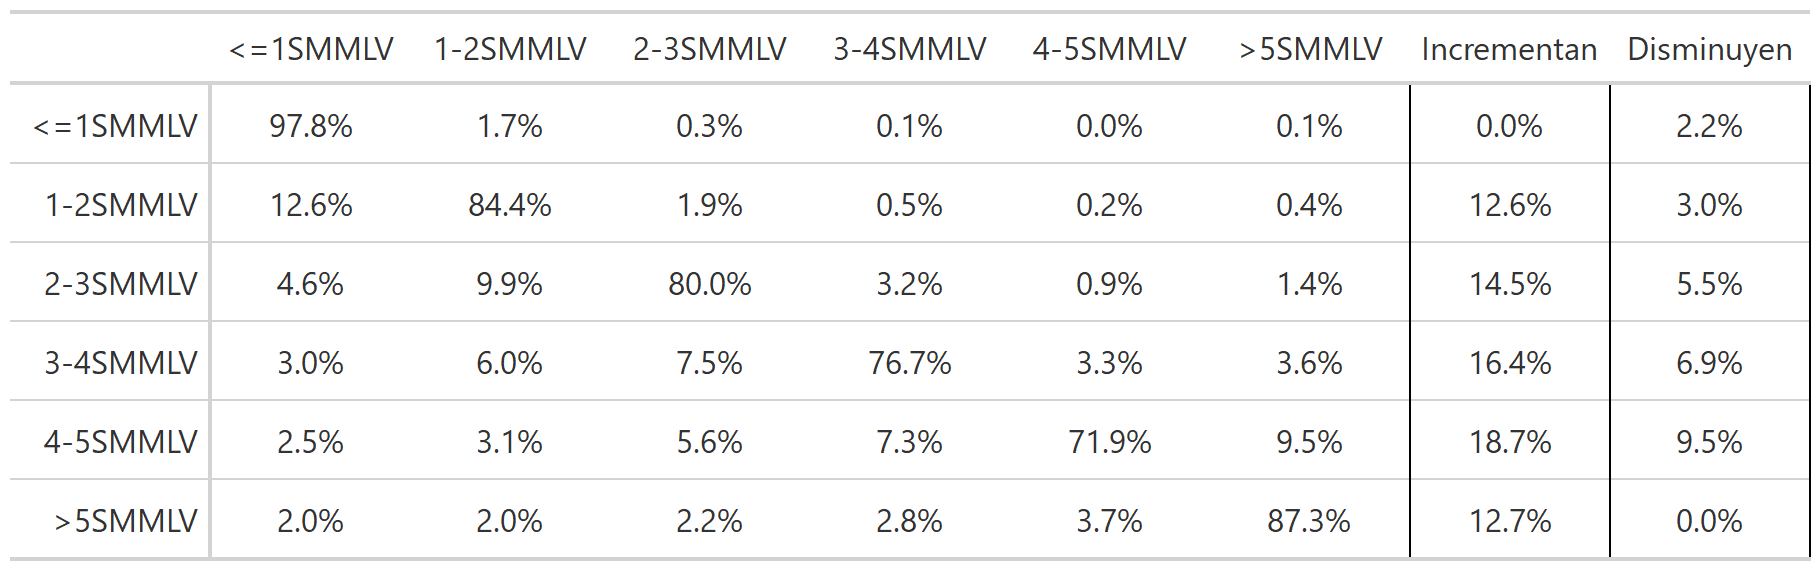
\includegraphics[width = 18cm]{results/02_longitudinal/salida_matriz_transicion_independientes_21.png}
\caption{Matriz de transición independientes Noviembre - Diciembre 2021}%
\label{tabla:independientes:actividad_economica}
\end{table}

\FloatBarrier
\paragraph{Análisis por sección económica}\mbox{}\\

\begin{table}[!htbp]
\centering
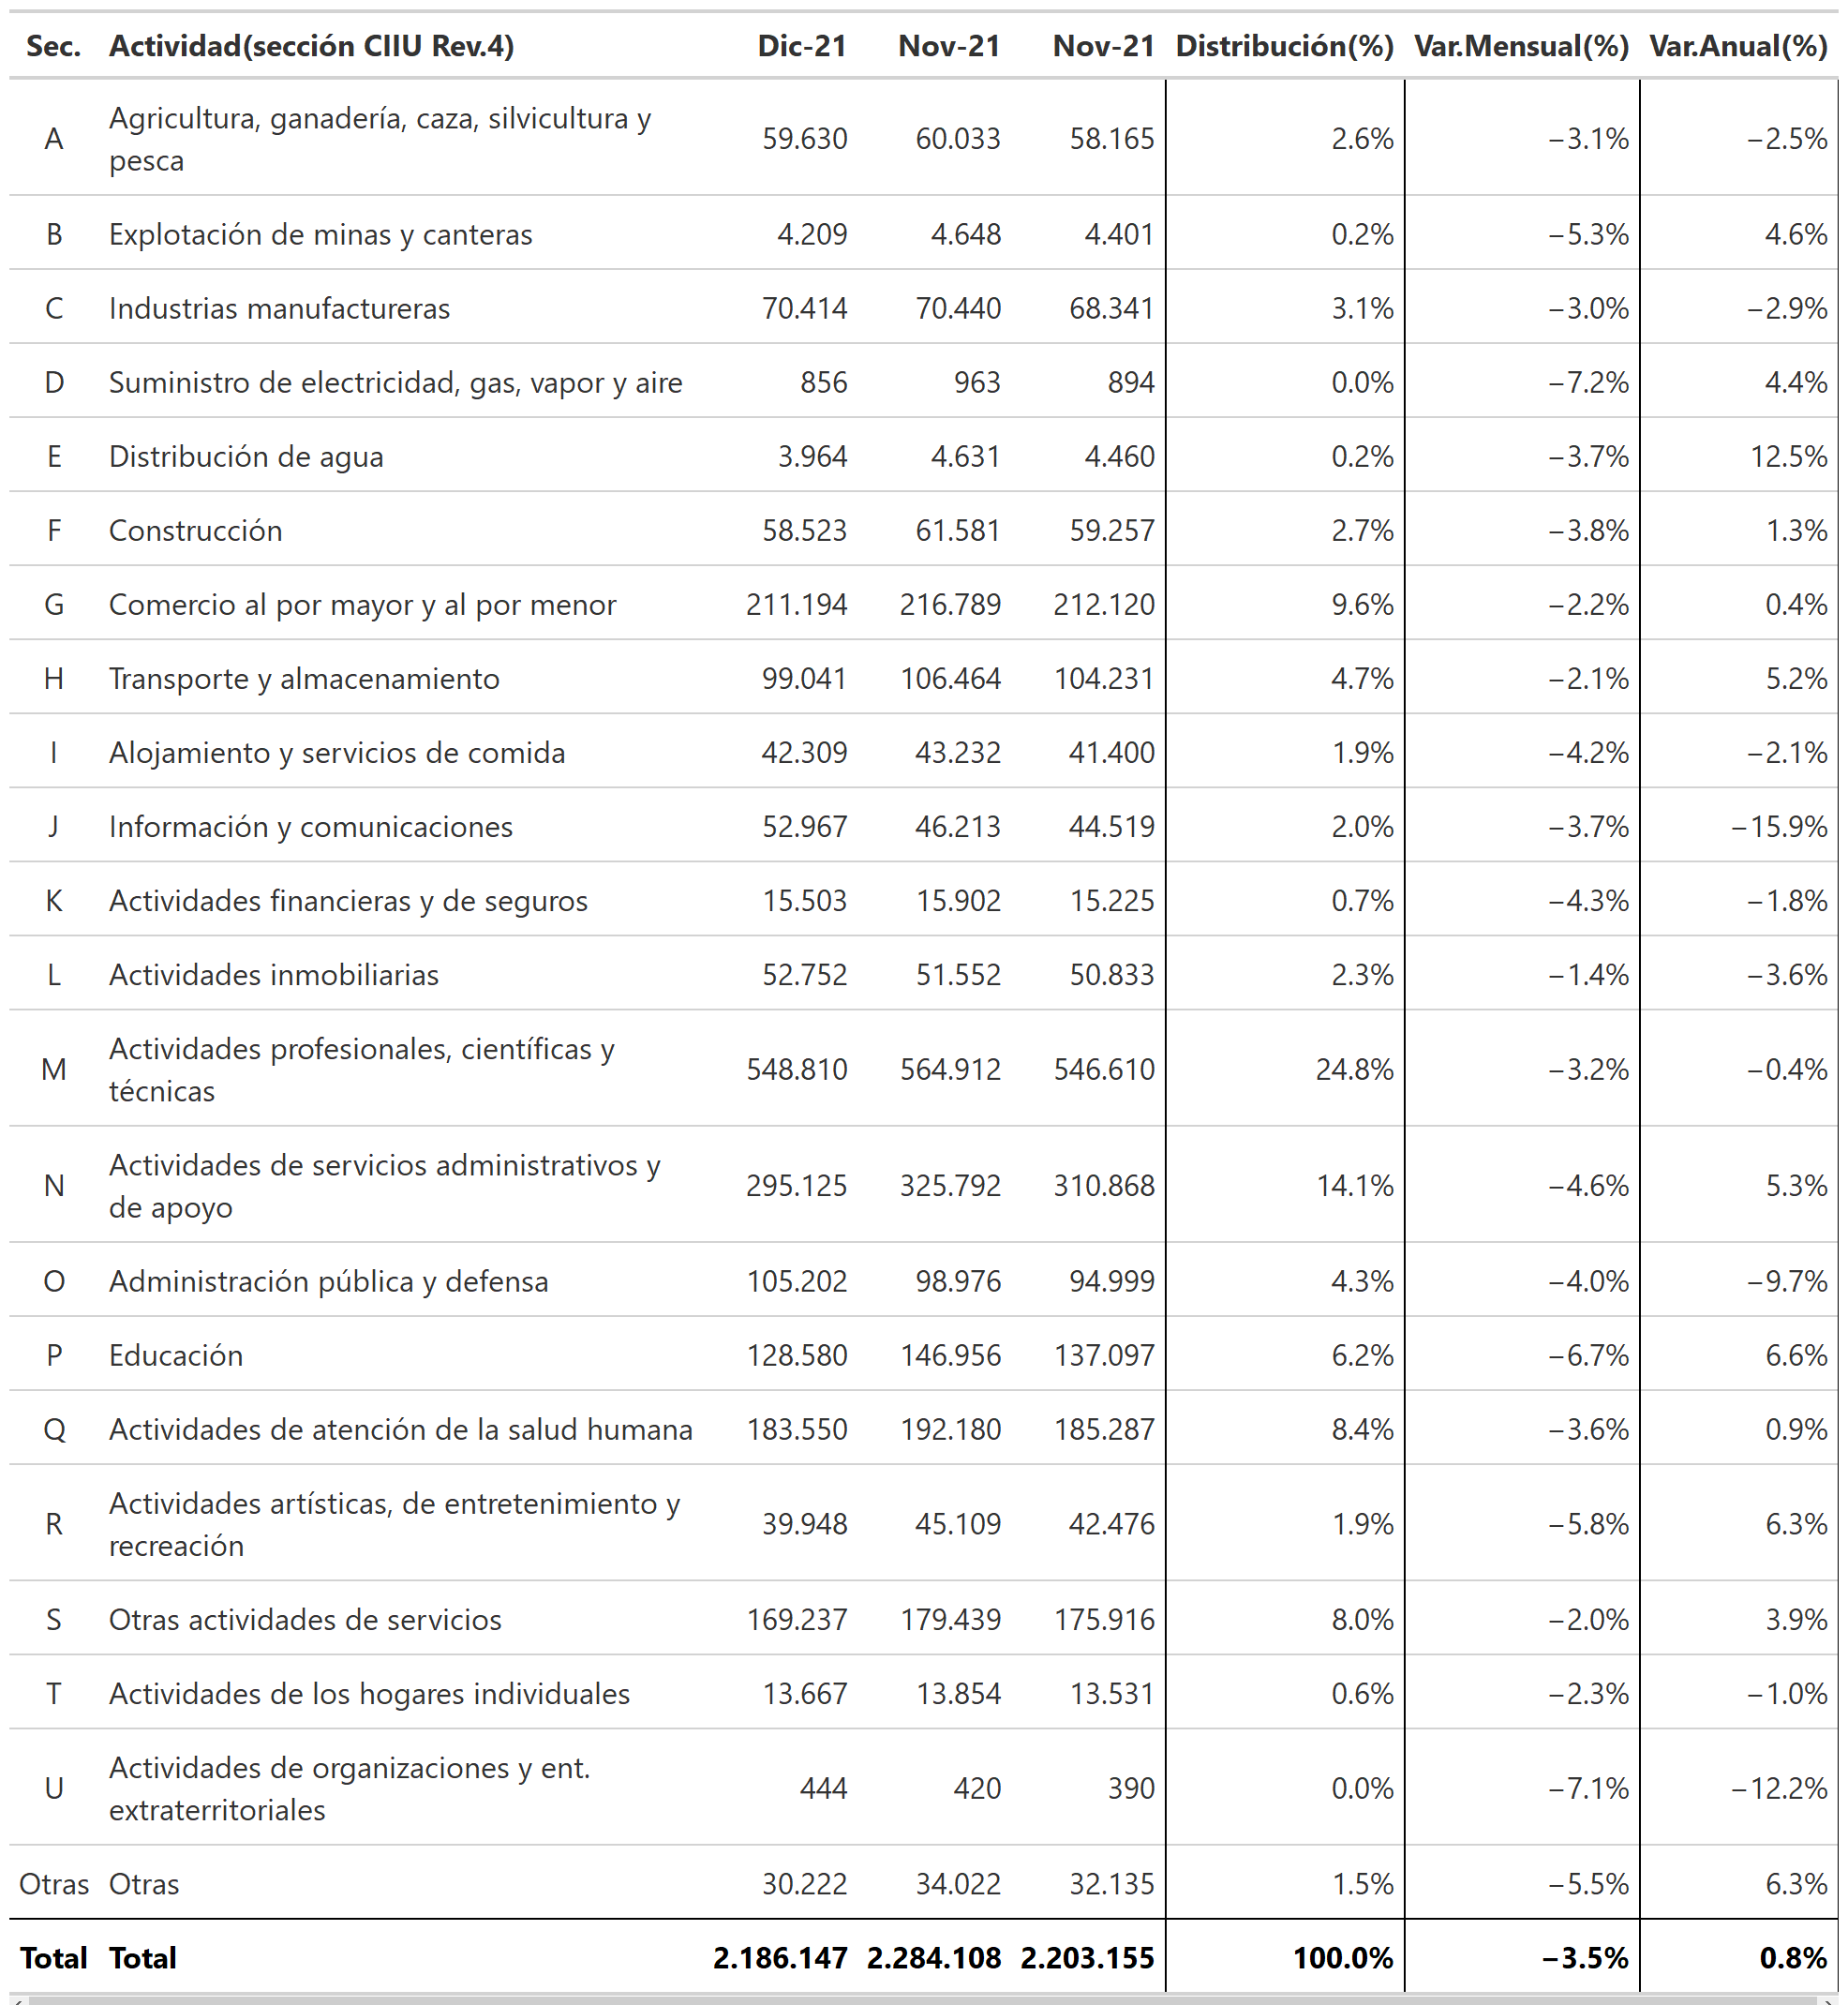
\includegraphics[width = 15cm]{results/02_longitudinal/salida_act_econ_independientes_21.png}
\caption{Total cotizantes independientes por sección económica}%
\label{tabla:independientes:actividad_economica}
\end{table}

\FloatBarrier
\subsection{Análisis demográfico dependientes sector privado e independientes}

\begin{figure}[!htbp]
\centering
\begin{minipage}{0.5\textwidth}
  \centering
  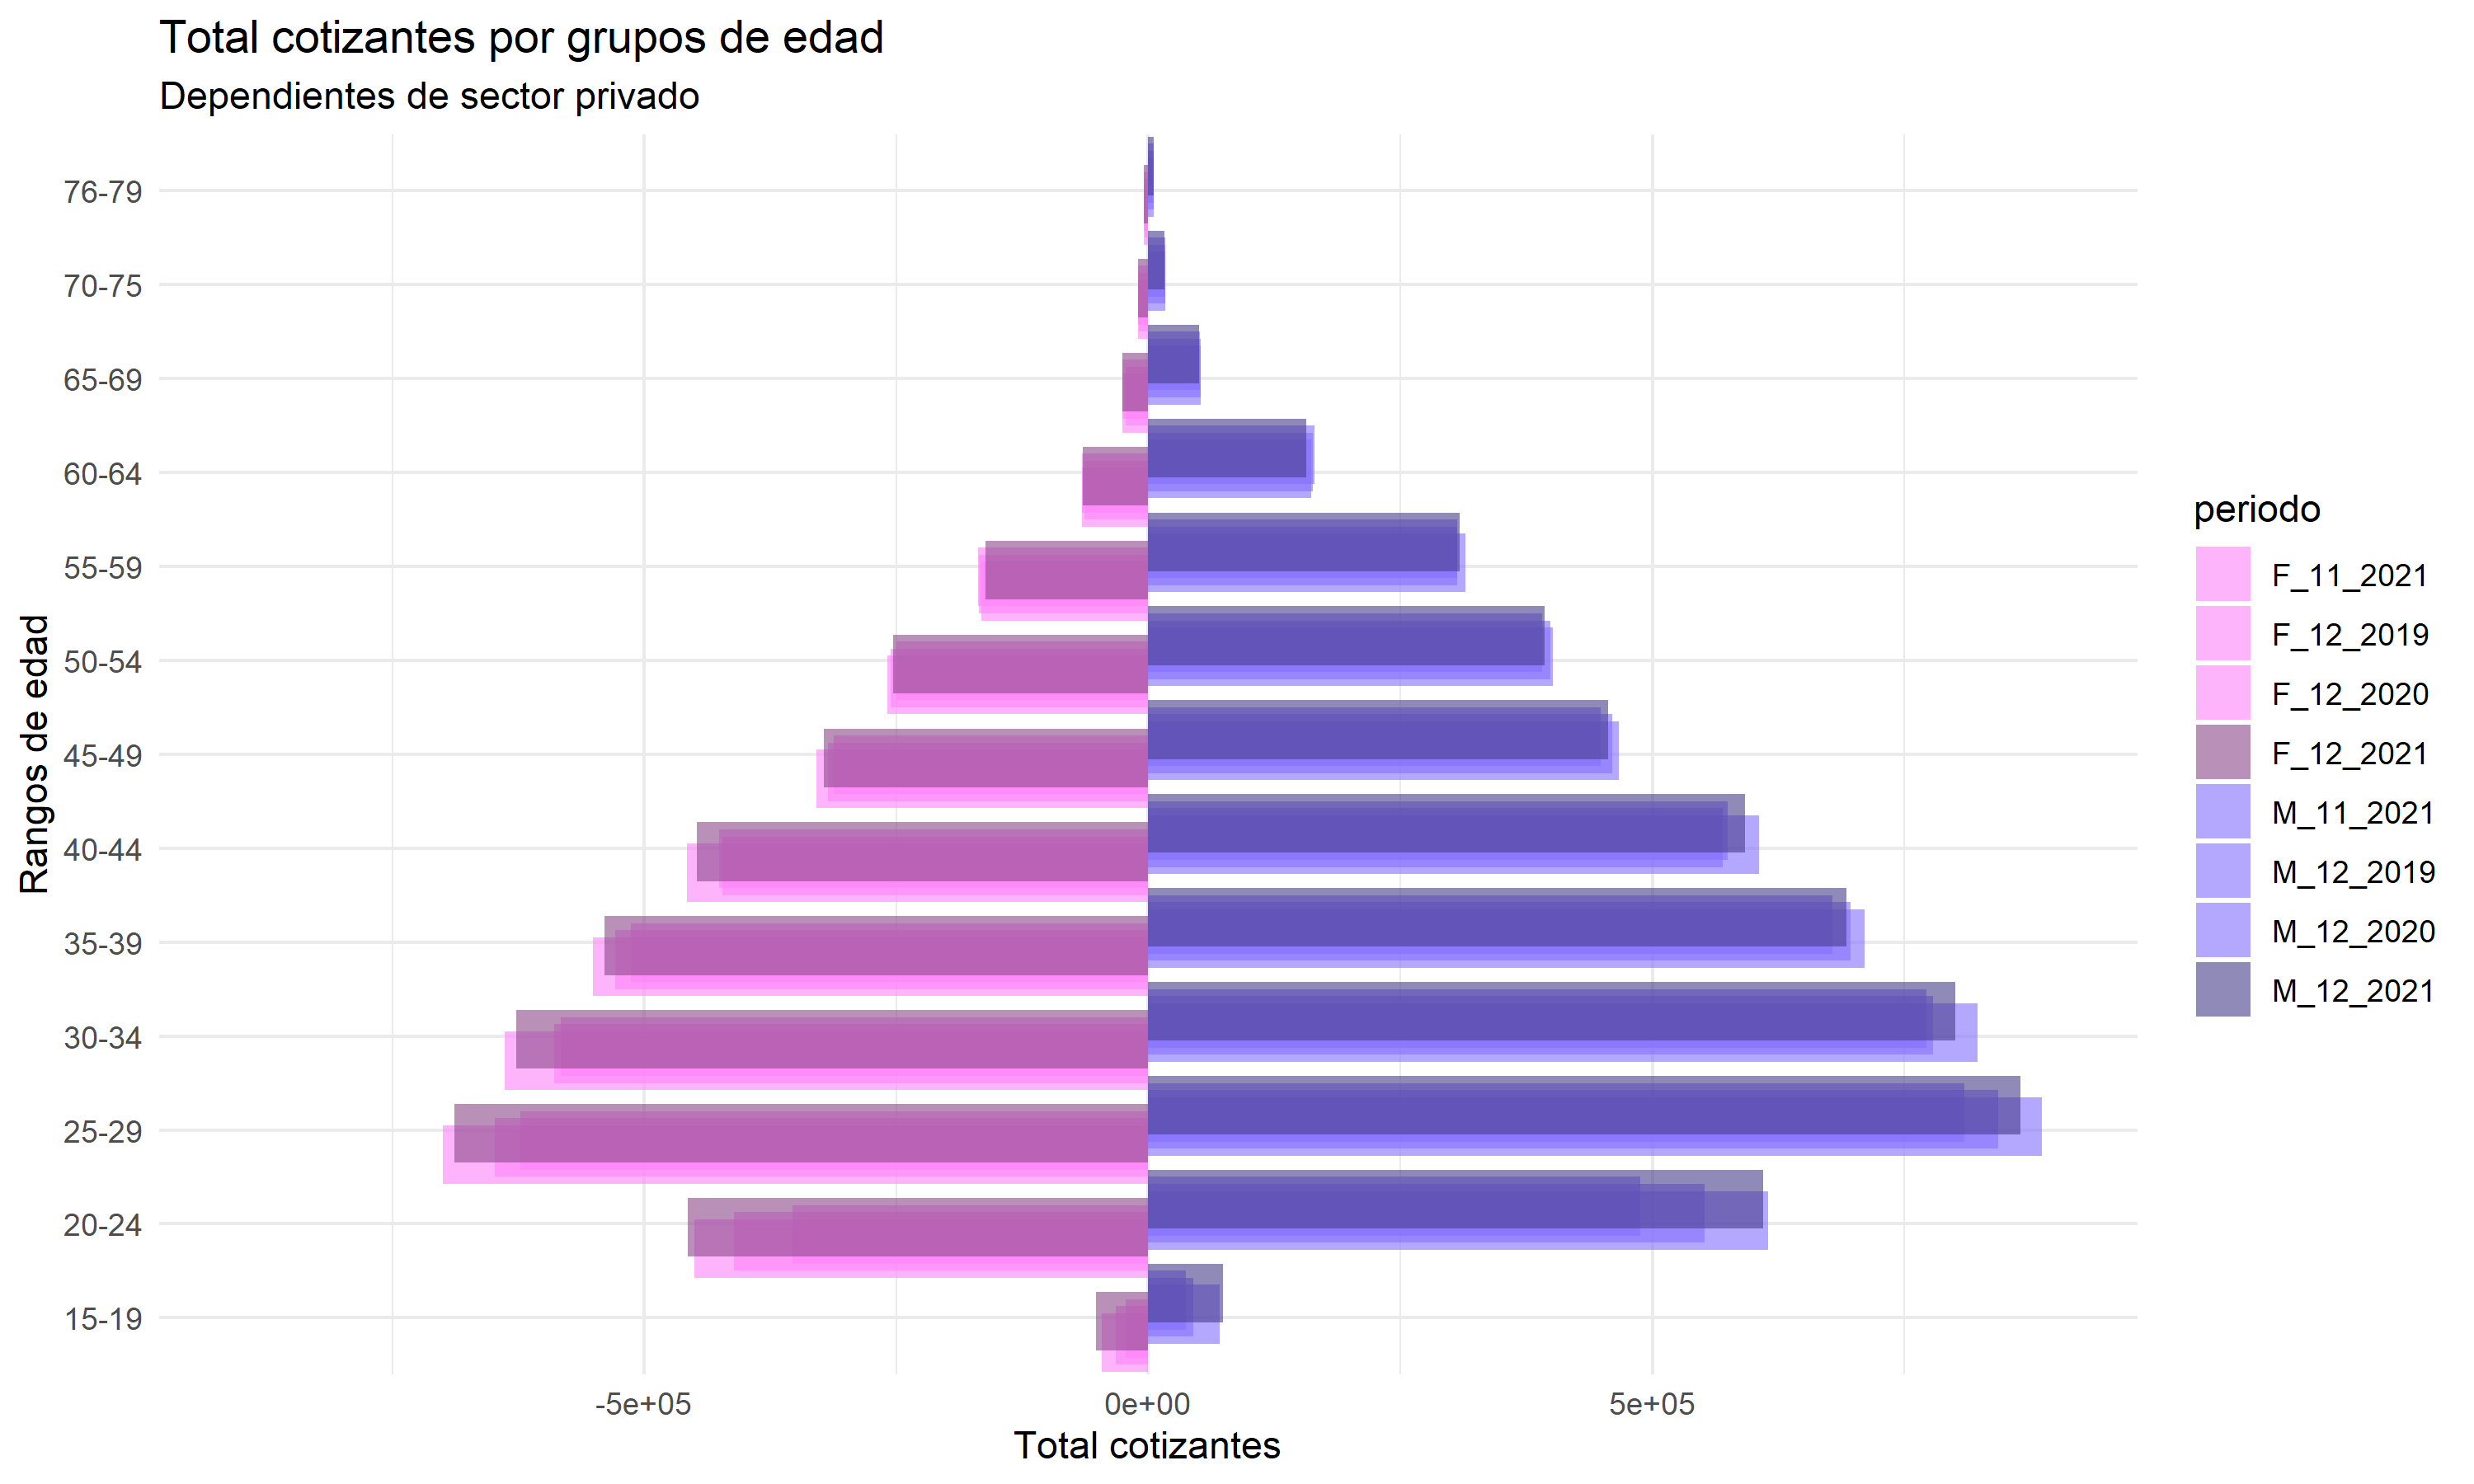
\includegraphics[width=\linewidth]{figures/02_longitudinal/salidas_piramide_dependientes.png}
\end{minipage}%
\begin{minipage}{0.5\textwidth}
  \centering
  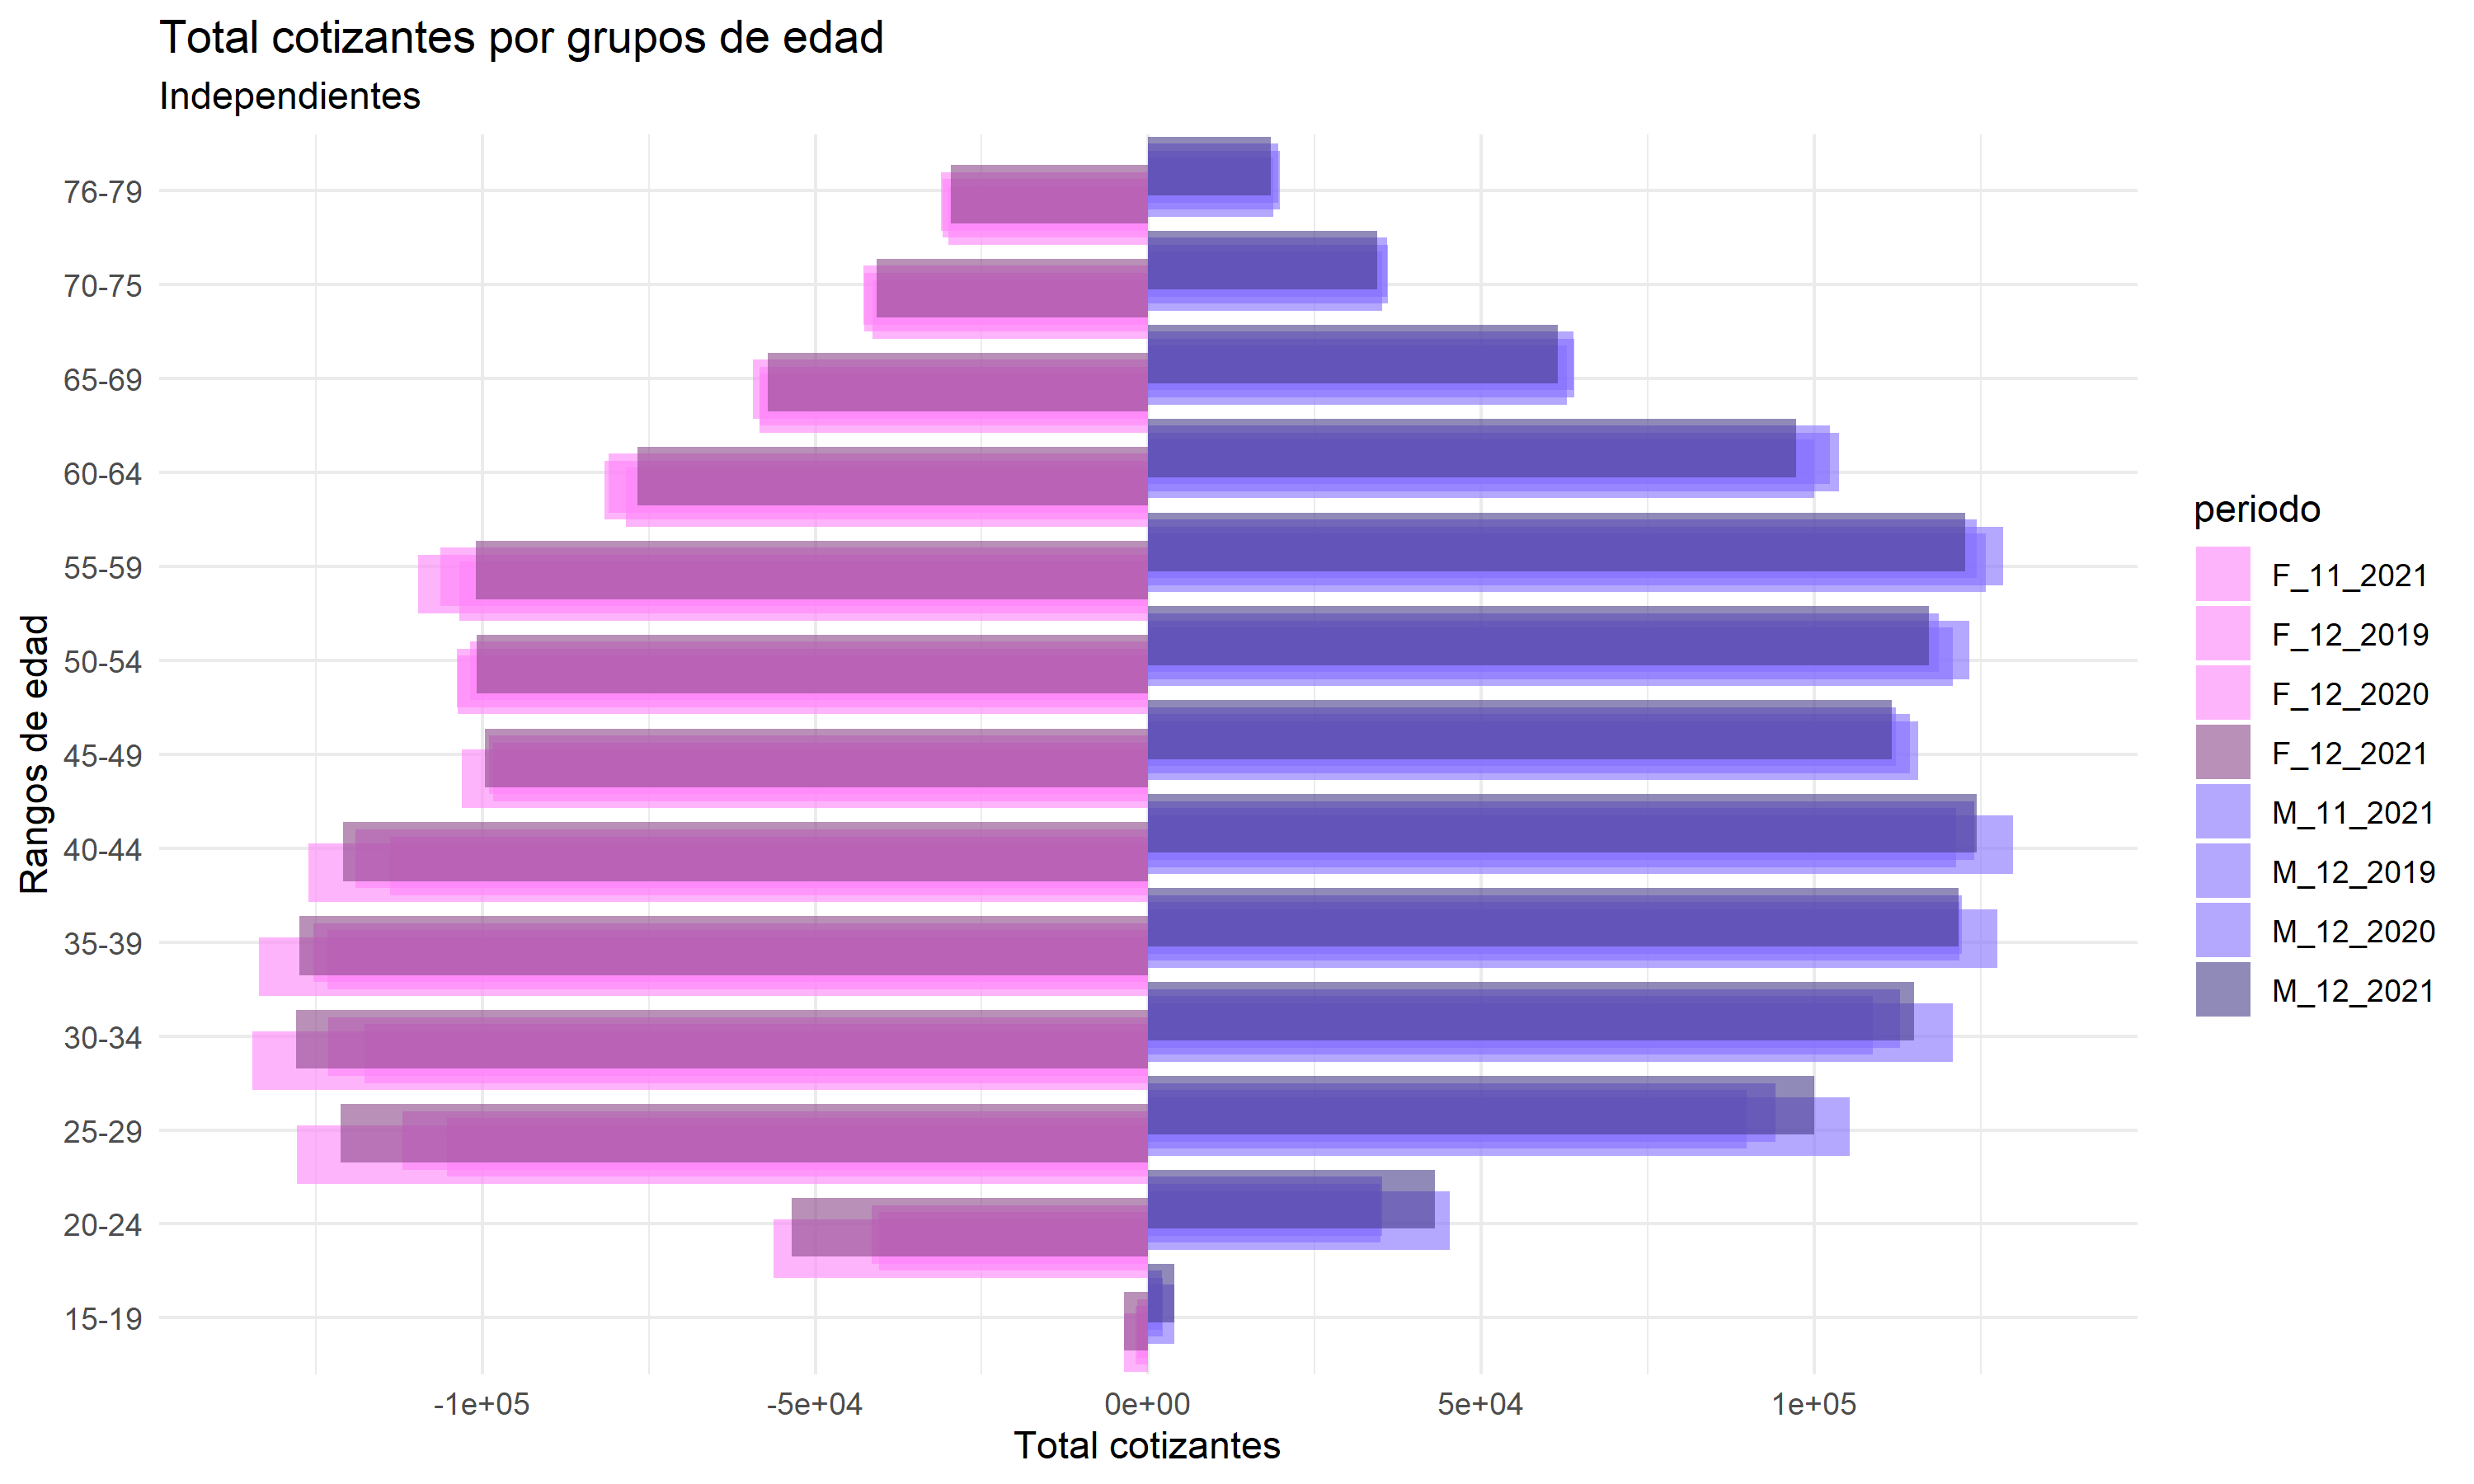
\includegraphics[width=\linewidth]{figures/02_longitudinal/salidas_piramide_independientes.png}
\end{minipage}
\caption{Porcentaje de entradas (izq.) y salidas (der.) por año}
\label{figura:piramides}
\end{figure}


